\chapter{Discusión }


En este capítulo se discuten y evalúan los resultados obtenidos.

\section{Comparación  de relaciones categoriales  de trabajos de grado de acuerdo a su dominio de conocimiento.}

En esta sección se evalúa las relaciones conceptuales taxonómicas o relaciones categoriales de los métodos propuestos en este trabajo. Dado que los trabajos de grado de este tipo de relaciones tienen rasgos comunes, las vinculaciones se establecen principalmente mediante mecanismos de detección de similitudes.

La medida de validación interna del agrupamiento, que se utiliza en este trabajo, consiste en determinar qué tan cohesionados están los grupos entre sí, se busca que los documentos relacionados de un mismo grupo se parezcan contextualmente más entre ellos que con los documentos de otros grupos; y por otra parte determinar qué tan separados son los documentos de un grupo con respecto a todos los documentos de otros grupos. 
Por tanto, la métrica que permite evaluar la agrupación de los dominios obtenidos es el coeficiente de Silhouette.

El coeficiente de Silhouette muestra qué documentos se encuentran completamente dentro de un grupo y cuáles han sido mal clasificados. Esta métrica tiene un rango de [-1, 1], un valor  mayor a 0 y cercano a 1 indica que el documento está lejos de los grupos vecinos, 0 indica que el documento está en o muy cerca de la frontera de decisión entre dos grupos vecinos, y valores negativos indican que el documento podría haber sido mal asignado al grupo.

\begin{table}[H]\centering
\caption{Validación Coeficiente de Silhouette algoritmo k medias para los conjuntos de datos generados }\label{tab:tablaeres}
	\begin{tabularx}{\textwidth}{XXXm{3.0cm}}\toprule

Modelo &  Coeficiente de Silhouette & K óptimo (20 –44)  \\
Doc2vec PV-DBOW & 0.36 & 32 \\
Doc2vec PV-DM &  0.34  & 27\\
Tf-idf 20000 variables & 0.04 & 38  \\
Tf-idf 10000 variables & -0.009 & 43 \\

 \bottomrule
	\end{tabularx}
\end{table}

En la tabla \ref{tab:tablaeres} se observa que el valor más alto de coeficiente de Silhouette está en los conjuntos generados por los modelos Doc2vec, por tanto  los algoritmos implementados en esta investigación se basaron en estos, particularmente en Do2vec PV-DBOW; ya que logra una mejor agrupación y separación de los dominós de conocimiento en el corpus de trabajos de grado de la universidad de Nariño.

\begin{figure}[H]\centering
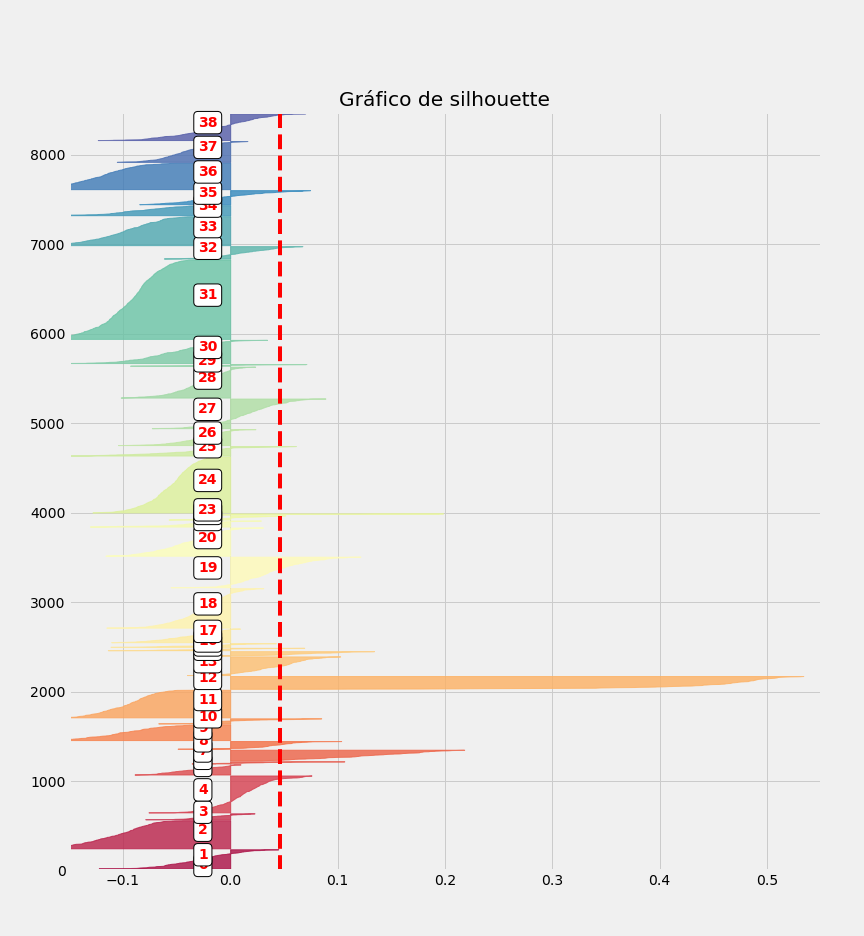
\includegraphics[width=0.8\textwidth]{CoefSilTFidf}
\caption{Gráfico de Silhouette algoritmo Kmedias con k=38 , Tf-idf 20000 variables}
\label{fig:siltfidf}
\end{figure}

En el gráfico de silhouette generado por el algoritmo Kmedias con k=38,Tf-idf 20000 variables, figura \ref{fig:siltfidf} se observa que la mayoría de los documentos del corpus fueron mal clasificados a su grupo ya que tienen un valor negativo de silhouette.

\begin{figure}[H]\centering
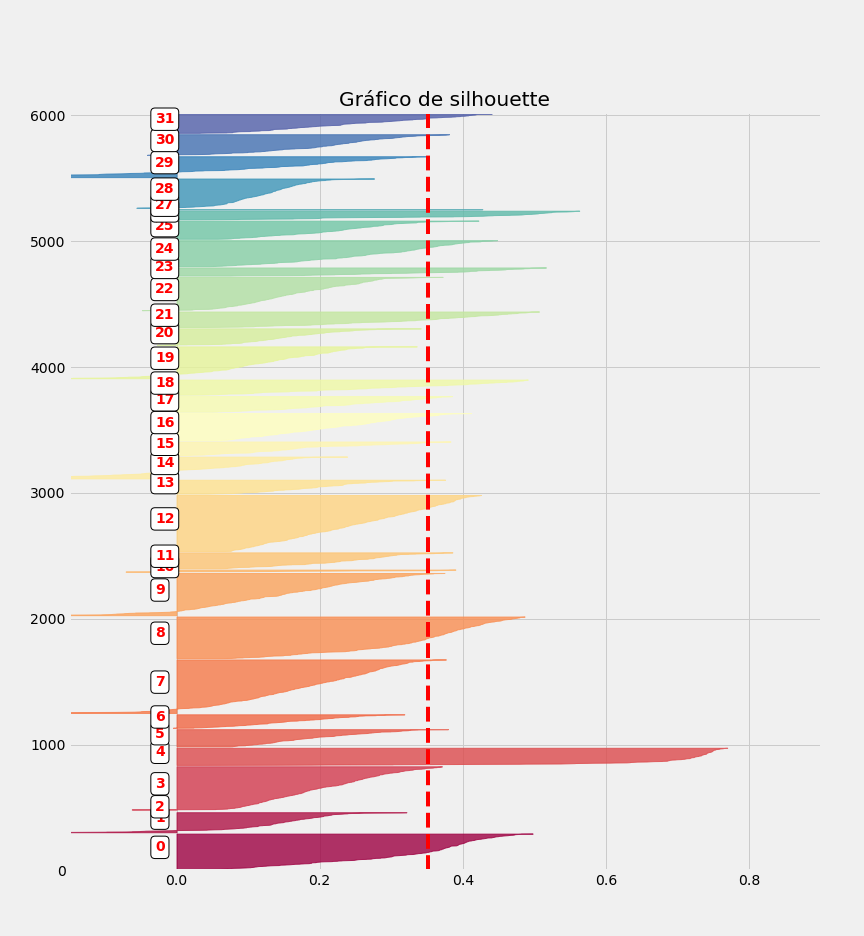
\includegraphics[width=0.8\textwidth]{CoefSilgeneral}
\caption{Gráfico de Silhouette algoritmo Kmedias con k=32 , método Doc2vec PV-DBOW}
\label{fig:sil1}
\end{figure}

 Por otro parte, en el gráfico de silhouette generado por el algoritmo Kmedias con k=32, método Doc2vec PVDBOW, figura \ref{fig:sil1} se observa que a pesar de existir documentos que quedaron mal clasificados; la gran mayoría de documentos están cohesionados de forma correcta a su respectivo grupo, Doc2vec tiene un rendimiento claramente superior a tf-idf por tanto es el método que se elige para relacionar trabajos de grado conceptualmente y generar recomendaciones.  


Contrastando con \cite{kim2019multi} lograron obtener mejores resultados ensamblando los modelos TF-IDF, IDA Y Doc2Vec , los resultados de la presente investigación de la tabla  \ref{tab:ProgramasDM} demuestran que los conjuntos estructurados con los métodos  TF-IDF  no tienen tendencia al agrupamiento por tal motivo este método quedó descartado para el repositorio de trabajos de grado.

En \cite{nandi2018bangla}  se observa que el método Doc2vec coincide en los resultados, reiterando que este tiene un mejor rendimiento y puede ser implementado en diferentes dominios de conocimiento.

 %%%%%%%%%%%%%%%%%%%%%%%%%%%%%%%%%%%%%%%%%%%%%%%%%%%%%%%%%%%%%%%%%%%%%%%%%%%%%%%%%%%%%%%%%%%%%%%%%%%%%%%%%%%%%%%%%%%%%%%%%%%%%%%%%%%%%%%%%%%%%%%%%%


%\section{Evaluación de trabajos de grado relacionados conceptualmente propuestos por Maskana.}
%
%Para la evaluación de los trabajos relacionados propuestos por el algoritmo Maskanita, se realizaron 3 casos de prueba, para los cuales se elaboró una tabla con los resultados obtenidos de las relaciones encontradas para diferentes trabajos de grado, para validar las relaciones propuestas por Maskanita se formaron dos grupos de trabajos; los que fueron relacionados por el algoritmo y los se quedaron por fuera de la frontera de decisión y no se relacionaron, para cada prueba se evalúa el coeficiente de silhouette y se valida la cohesión de los trabajos relacionados y la separación con respecto al grupo de trabajos que no se relacionaron.
%
%
%\begin{table}[H]\centering
%\caption{Caso de prueba 1: Resultados recomendación para el trabajo de grado Tariykdd: Una herramienta genérica de descubrimiento de conocimiento en bases de datos débilmente acoplada con el sgbd Postgresql.}\label{tab:tablae1}
%	\begin{tabularx}{\textwidth}{XXXm{3.0cm}}\toprule
%
%Id &  \multicolumn{1}{c}{Distancia Milikowski } & \multicolumn{1}{c}{Titulo} \\ 
%5268 &0.0006 &Pg\_KDD - Entorno Gráfico para el Sistema de Descubrimiento de 
%Conocimiento en Bases de Datos PostgresKDD.   \\ 
%446 &  0.0007 &Implantación de primitivas sql para el descubrimiento de reglas de asociación y clasificación al interior del motor del sistema gestor de bases de datos postgresql.   \\ 
%183 & 0.0033 &MATE-KDD: Una herramienta genérica para el descubrimiento.   \\ 
%4081 &0.0097&EXDACLET: Herramienta de datacleaning basada en agentes inteligentes orientadas a la web \\
%
% \bottomrule
%	\end{tabularx}
%	
%\end{table}
%
%\begin{table}[H]\centering
%\label{tab:tablae1}
%	\begin{tabularx}{\textwidth}{XXXm{3.0cm}}\toprule
%
%%Id &  \multicolumn{1}{c}{Distancia Milikowski } & \multicolumn{1}{c}{Titulo} \\ 
%4130 & 0.0363  &RASEMUS: Una herramienta para el descubrimiento de conocimiento en bases de datos con técnicas de clustering, débilmente acoplado con el sgbd postgresql. \\ 
%6975&0.1320&POLARIS: Herramienta de minería de uso para la web. \\
%6206&0.1537&GRFPOSTGRES – Herramienta gráfica para el motor de base de datos postgres.\\
%5044&0.1555&STARCUBE: Una herramienta ROLAP de análisis multidimensional para el soporte a la toma de decisiones, débilmente acoplada con el SGBD PostgreSQL. \\
% \bottomrule
%	\end{tabularx}
%	
%\end{table}
%
%\begin{figure}[H]\centering
%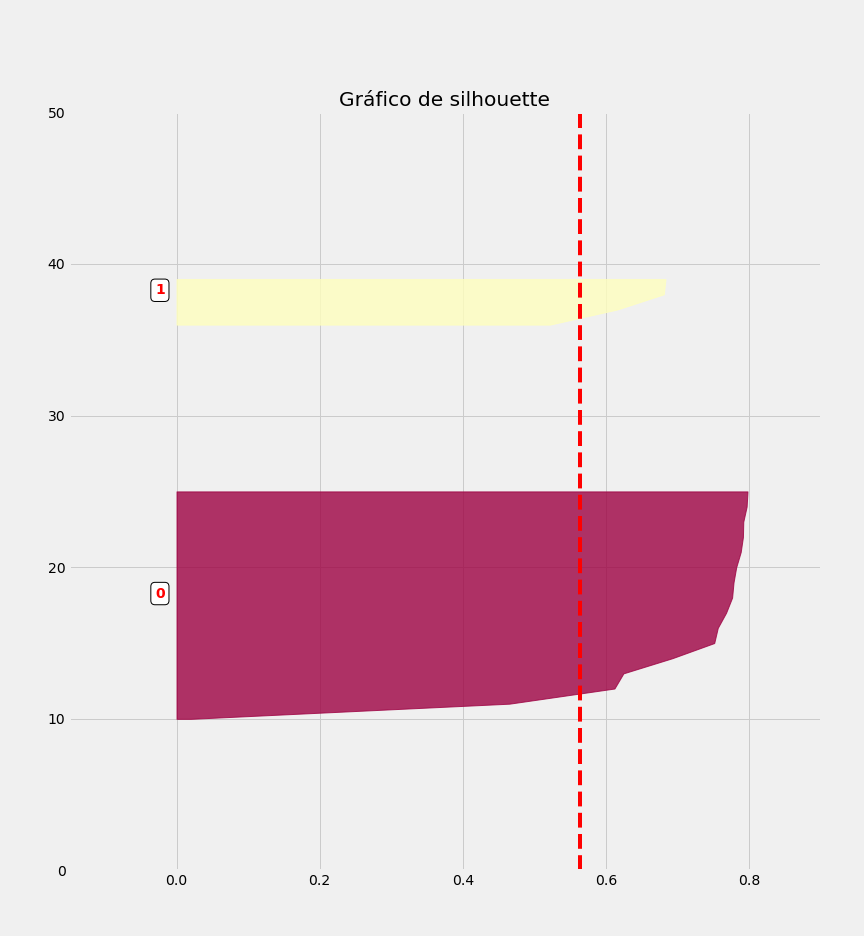
\includegraphics[width=0.8\textwidth]{CoefSil1}
%\caption{Gráfico de Silhouette recomendación caso de prueba 1 }
%\label{fig:silruno}
%\end{figure}
%
%
%
%
%\begin{table}[H]\centering
%\caption{Caso de prueba 2: Resultados recomendación para el trabajo de grado Desarrollo e implementación de un sistema de reconocimiento de comandos de voz basado en redes neuronales para la activación de dispositivos electrónicos.}\label{tab:tablae2}
%	\begin{tabularx}{\textwidth}{XXXm{3.0cm}}\toprule
%
%Id &  \multicolumn{1}{c}{Distancia Milikowski } & \multicolumn{1}{c}{Titulo} \\ 
%5268 &0.0066 &Sistema interactivo de reconocimiento de fonemas para la interpretación de voz y traducción a lengua de señas.  \\ 
%446 &  0.0067 &Implementación de redes neuronales artificiales en hardware reconfigurable.Implementación de redes neuronales artificiales en hardware reconfigurable.   \\ 
%183 & 0.0087 &Análisis de deformaciones debidas a esfuerzos, vibraciones o variaciones de temperatura en un objeto mediante metrología óptica basada en técnicas de interferometría holográfica.   \\ 
%4081 &0.0122&Diseño e implementación de un sistema que activa dispositivos electrónicos mediante señales oculares para mejorar la comunicación a personas con discapacidad motora. \\
%4130 & 0.0314  &Detección automática de registros sísmicos asociados al comportamiento del volcán galeras haciendo uso de redes. \\ 
%
% \bottomrule
%	\end{tabularx}
%	
%\end{table}
%
%
%\begin{table}[H]\centering
%\label{tab:tablae2}
%	\begin{tabularx}{\textwidth}{XXXm{3.0cm}}\toprule
%
%%Id &  \multicolumn{1}{c}{Distancia Milikowski } & \multicolumn{1}{c}{Titulo} \\ 
%6975&0.0395&Evaluar un acople colimador fibra óptica para valorar su comportamiento como medidor de intensidad luminosa. \\
%6206&0.0476&Optimización de un sistema de control para la navegación basado en el método de campo de fuerza virtual para un vehículo autónomo empleando algoritmos genéticos.\\
%5044&0.0526&Diseño e implementación de un sistema portátil de registro de señales micro-sísmicas. \\
%5044&0.0648&Identificación de aves a partir de canto característico e información contenida en bases de datos. \\
%5044&0.0786&Diseño e implementación del prototipo de un osciloscopio. \\
%
% \bottomrule
%	\end{tabularx}
%	
%\end{table}
%
%\begin{figure}[H]\centering
%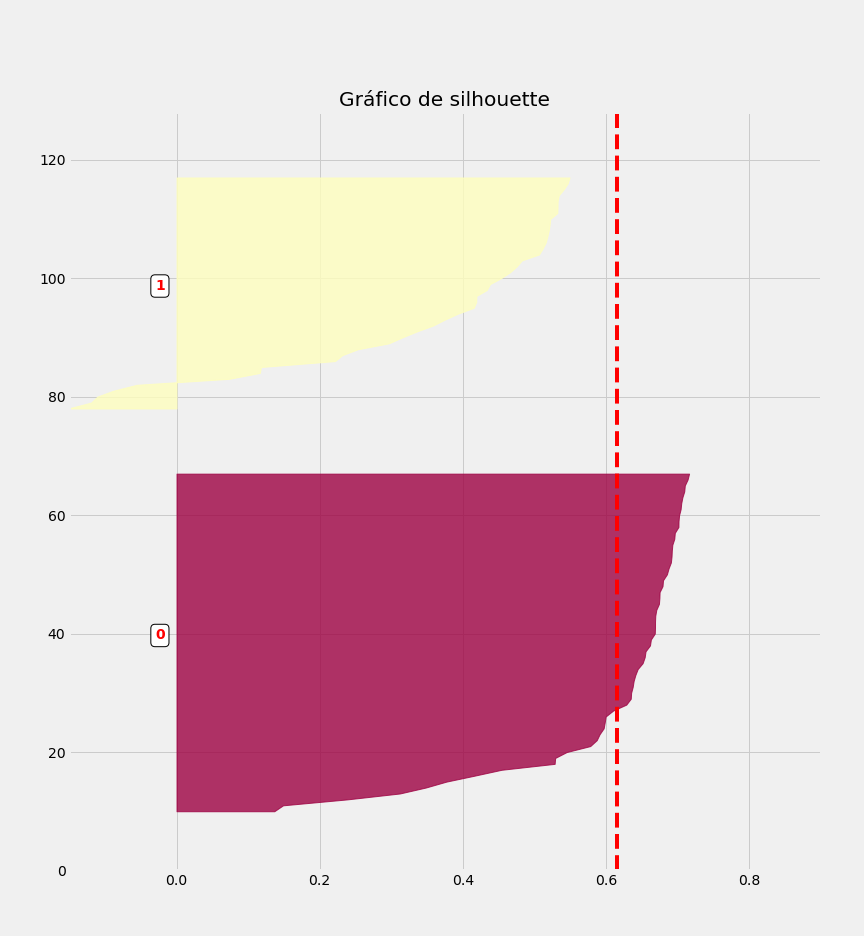
\includegraphics[width=0.8\textwidth]{CoefSil2}
%\caption{Gráfico de Silhouette recomendación caso de prueba 2 }
%\label{fig:silrdos}
%\end{figure}
%
%\begin{table}[H]\centering
%\caption{Caso de prueba 3: Resultados recomendación para el trabajo de grado Construcción de un repositorio limpio de datos para la detección de patrones de eventos eruptivos del volcán galeras con técnicas de minería de datos.}\label{tab:tablae3}
%	\begin{tabularx}{\textwidth}{XXXm{3.0cm}}\toprule
%
%Id &  \multicolumn{1}{c}{Distancia Milikowski } & \multicolumn{1}{c}{Titulo} \\ 
%5268 &0.0685 &Detección automática de registros sísmicos asociados al comportamiento del volcán galeras haciendo uso de redes neuronales artificiales.  \\ 
%446 & 0.1015 &Monitoreo electromagnético de volcanes.   \\ 
%183 & 0.1615 &Implementación de un método fundamentado en la distribución de amplitudes para la localización de sismos asociados al movimiento de fluidos en el volcán galeras, Colombia.   \\ 
%4081 &0.3012&Diseño e implementación de estación modelo de registro, trasmisión y recepción de eventos micro-sísmicos de la red sísmica de san juan de pasto. \\
%4130 & 0.3286&Diseño e implementación del prototipo de una estación meteorológica automática portátil capaz de transmitir los datos mediante tecnología gsm. \\ 
%
% \bottomrule
%	\end{tabularx}
%	
%\end{table}
%
%\begin{figure}[H]\centering
%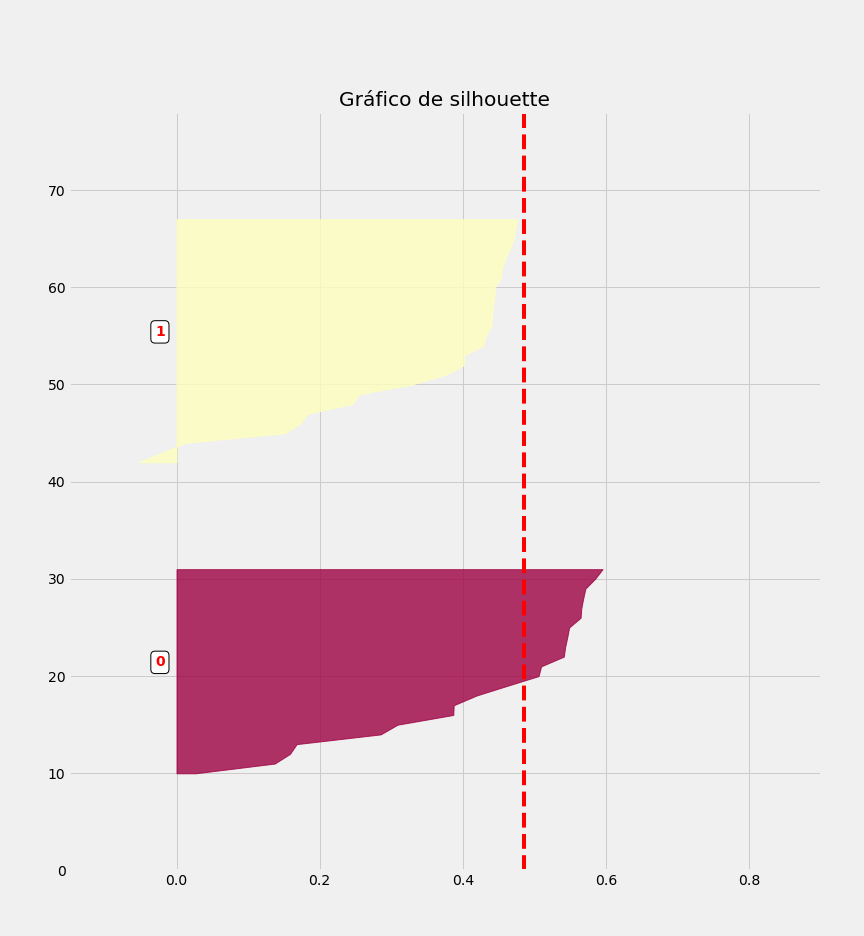
\includegraphics[width=0.8\textwidth]{CoefSil3}
%\caption{Gráfico de Silhouette recomendación caso de prueba 3 }
%\label{fig:silrtres}
%\end{figure}
%
%
%En las figura \ref{fig:silruno}, \ref{fig:silrdos} y ~\ref{fig:silrtres} se puede apreciar que los documentos relacionados propuestos por Maskanita (color rojo) están cohesionados de forma correcta a su grupo, ya que no se observan valores de silueta negativos, los valores promedio de silhouette para los 3 casos son de 0.58, 0.62 y 0.5 respectivamente; indicando  que los grupos se ajustan adecuadamente, en las ~\ref{fig:silrdos} y  ~\ref{fig:silrtres} se puede observar algunos valores de silhouette negativos en el grupo de documentos que no fueron relacionados por Maskanita (color amarillo), lo cual indica que no se cohesionan correctamente, ya que podría existir un tercer grupo o tercer dominio donde estos se agrupen adecuadamente; lo cual no es de importancia ya que la atención se centra en el grupo de documentos relacionados por el método implementado.

%\section{Interpretación de las categorías  mediante grafos conceptuales.}
%
%En esta sección se interpreta el conocimiento obtenido mediante grafos conceptuales, los cuales permiten visualizar relaciones conceptuales temáticas; organizando contextualmente el corpus de trabajos de grado; soportadas por el modelo Word2vec, estos fueron elaborados para trabajos de grado relacionados encontrados en diferentes áreas de conocimiento de cada grupo formado.
%En la figura \ref{fig:procesocinco} se observa la distribución de los diferentes documentos del repositorio; estructurados por el modelo Doc2vec con su respectivo grupo en coordenadas de las componentes principales. A continuación, se interpreta cada grupo y el dominio de conocimiento que representa.
%
%\begin{figure}[H]
%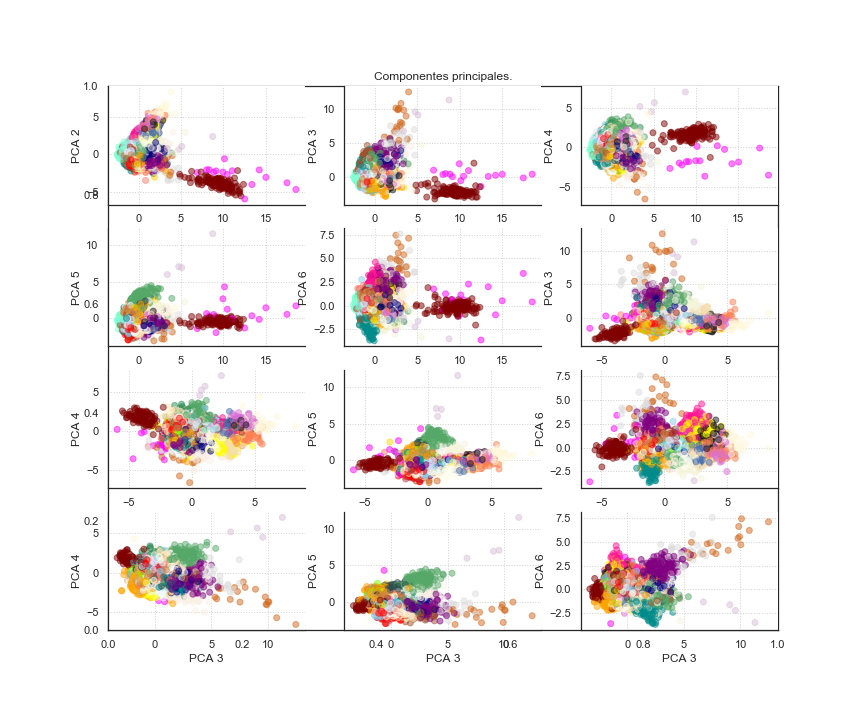
\includegraphics[width=1\textwidth]{proceso5}
%\caption{Biplot componentes principales}
%\label{fig:procesocinco}
%\end{figure}
%
%En el grupo 0 se encuentran trabajos relacionados a temáticas respectivas a los derechos humanos, derechos constitucionales, derechos laborales, derechos penales, derecho judicial, derecho administrativo, leyes y artículos constitucionales.
%En el grupo 1 se encuentran trabajos de grado relacionados a temáticas de desempleo, desigualdad social , condiciones socioeconómicas, fortalecimiento del comercio y economía. 
%En el grupo 2 se encuentran trabajos relacionados a temáticas de relaciones interfamiliares, estudios de violencia, conflictos familiares, machismo, patriarcado y problemáticas dentro del contexto sociológico como describe la figura \ref{fig:grupo14}.
%\begin{figure}[H]\centering
%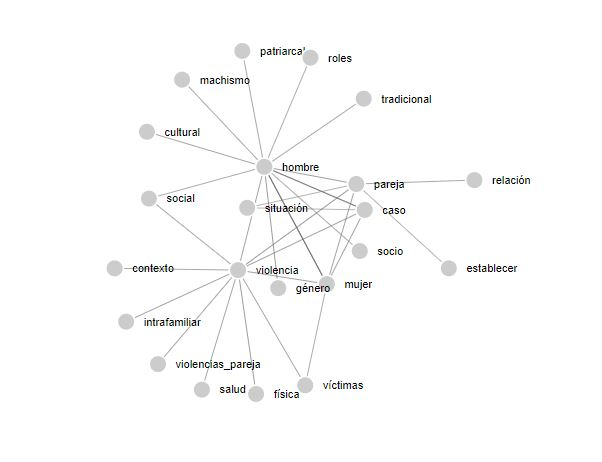
\includegraphics[width=0.8\textwidth]{grupo14}
%%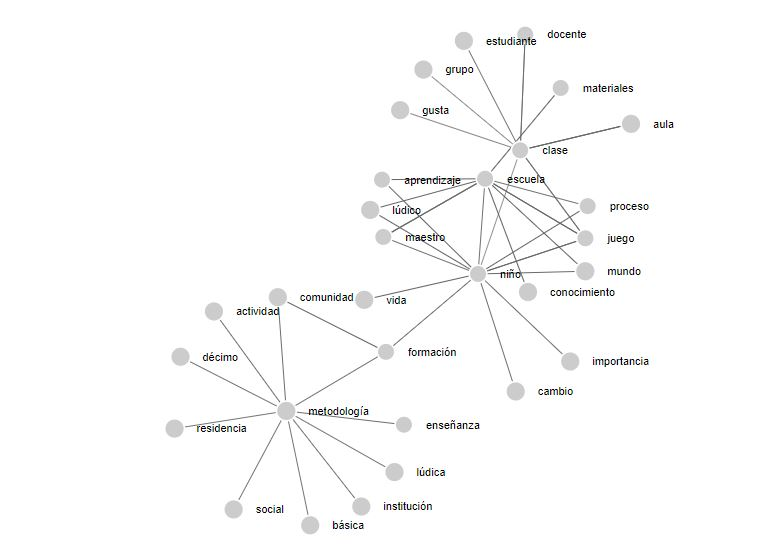
\includegraphics[width=0.8\textwidth]{grupo8}
%\caption{Grafo  relaciones temáticas grupo 2 }
%\label{fig:grupo14}
%\end{figure}
%
%%En el grupo 8 se encuentran trabajos relacionados con temáticas pedagógicas para la educación básica primaria. 
%%\begin{figure}[H]\centering
%%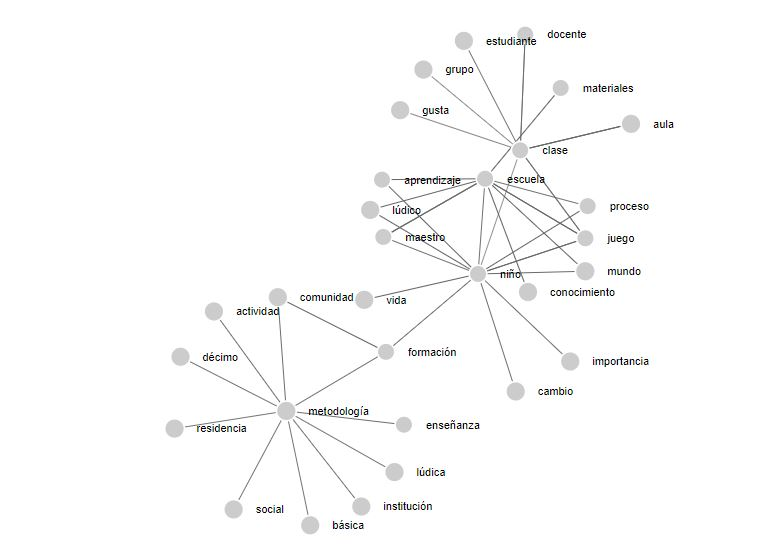
\includegraphics[width=0.8\textwidth]{grupo8}
%%\caption{Grafo  relaciones temáticas  grupo 8 }
%%\label{fig:grupo8}
%%\end{figure}
%
%%En la figura \ref{fig:grupo14} podemos observar relaciones contextuales complementarias del grupo 8 tales como: escuela, maestros , aulas de clase, estrategias y metodologías didácticas de aprendizaje basadas en lúdicas y juegos para niños estudiantes de básica  primaria.
%
%En el grupo 3 se encuentran trabajos de grado relacionados a temáticas de planeación estratégica empresarial, marketing y estudios de comercio en  organizaciones, como se puede observar en la figura \ref{fig:grupo5} .
%\begin{figure}[H]\centering
%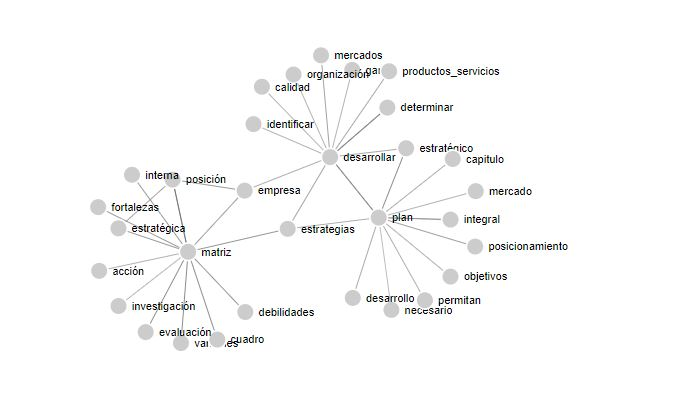
\includegraphics[width=1\textwidth]{grupo5}
%\caption{Grafo relaciones temáticas grupo 3 }
%\label{fig:grupo5}
%\end{figure}
%
%En el grupo 4 se encuentran trabajos de grado relacionados al departamento de idiomas, todos los documentos de este grupo se encuentran en idioma inglés, reprentado en la figura \ref{fig:grupo6}.
%
%\begin{figure}[H]\centering
%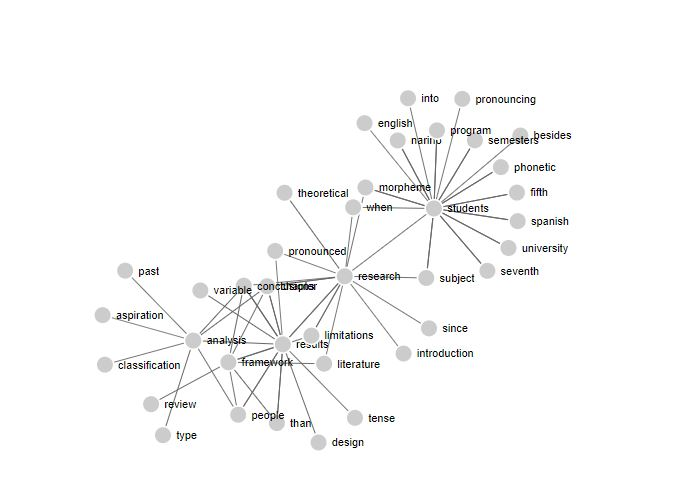
\includegraphics[width=0.8\textwidth]{grupo6}
%\caption{Grafo  relaciones temáticas grupo 4 }
%\label{fig:grupo6}
%\end{figure}
%
%En el grupo 5 se encuentran trabajos de grados vinculados a la facultad de ciencias exactas, específicamente al programa de Biología, evaluando diferentes tratamientos para encontrar diferencias estadísticamente significativas entre estos y así mejorar el crecimiento y producción de especies. %%
%
%En el grupo 6 se encuentran trabajos relacionados al estudio de modelamiento de fluidos.
%
%En el grupo 7 se encuentran trabajos de grado relacionados a temas de cultura, carnavales, historia y desarrollo social.
%\begin{figure}[H]\centering
%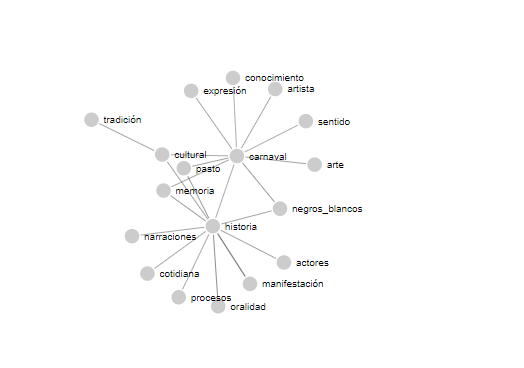
\includegraphics[width=0.8\textwidth]{grafocul0}
%\caption{Grafo  relaciones temáticas grupo 7 }
%\label{fig:grafoculcero}
%\end{figure}
%
%
%
%La figuera \ref{fig:grafoculcero}  se muestra el grafo  conceptual  de los trabajos de grado clasificados en el grupo 7, donde se observa conceptos relacionados referentes al carnaval de negros y blancos, cultura, artes , maestros y artesanos.
%
%En el grupo 8 se encuentran trabajos relacionados a construcción, desarrollo, gestión de calidad y auditoría de obras civiles.
%
%En el grupo 9 se encuentran trabajos de grado relacionados con temáticas pedagógicas de aprendizaje   y estrategias lúdicas de aprendizaje  para estudiantes.
%
%En el grupo 10 se encuentran trabajos de grado relacionados específicamente a ingeniería de software, lenguaje unificado de modelado UML, desarrollo y construcción de módulos y sistemas de información a la medida.
%
%En el grupo 11 se encuentran trabajos relacionados a telemática, microcontroladores, reconocimiento de imágenes, redes neuronales ,  espectro electromagnético,  series temporales,  aplicaciones en vulcanología y sismología. 
%
%En el grupo 12 se encuentran trabajos de grado vinculados al programa de ingeniería agroindustrial referentes a temáticas de desarrollo, comercialización, industrialización, estudios de oferta y demanda de productos agropecuarios.
%
%En el grupo 13 se encuentran trabajos de grado en temáticas de ordenamiento territorial, desarrollo sostenible y seguridad social.  %%%%%
%
%En el grupo 14 se encuentran trabajos de grado relacionados con proyectos referentes a entornos y herramientas virtuales de aprendizaje.
%
%En el grupo 15 se encuentran trabajos de grado vinculados a esquemas de seguridad, salud ocupacional en la industria y riesgos laborales como se describe en la figura \ref{fig:grupo22}
%
%
%\begin{figure}[H]\centering
%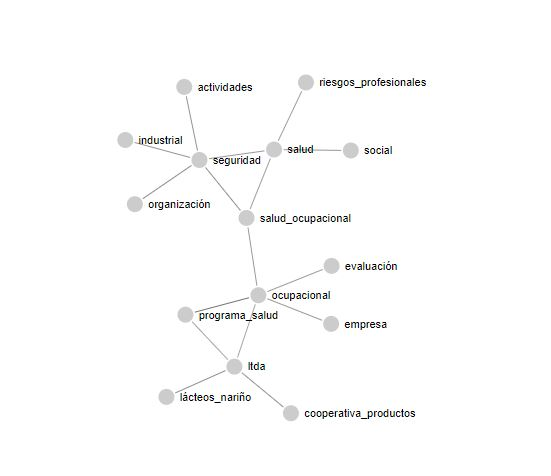
\includegraphics[width=0.8\textwidth]{grupo22}
%\caption{Grafo  relaciones temáticas grupo 15}
%\label{fig:grupo22}
%\end{figure}
%
%
%En el grupo 16 se encuentran trabajos de grado relacionados a cultivos, recursos hídricos  , plantas, especies y temáticas agroforestales como se observa en la figura \ref{fig:grupo1especies}.
%\begin{figure}[H]\centering
%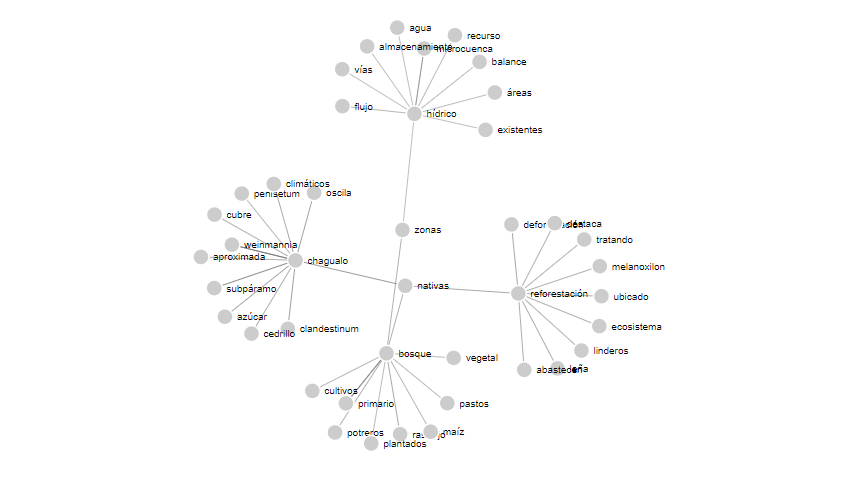
\includegraphics[width=1\textwidth]{grupo1especies}
%\caption{Grafo relaciones temáticas grupo 16 }
%\label{fig:grupo1especies}
%\end{figure}
%
%El grupo 17 contiene tópicos relacionados con bacterias, microorganismos, compuestos antioxidantes, proteínas y aminoácidos como se describe en la figura \ref{fig:grupo25}.
%\begin{figure}[H]\centering
%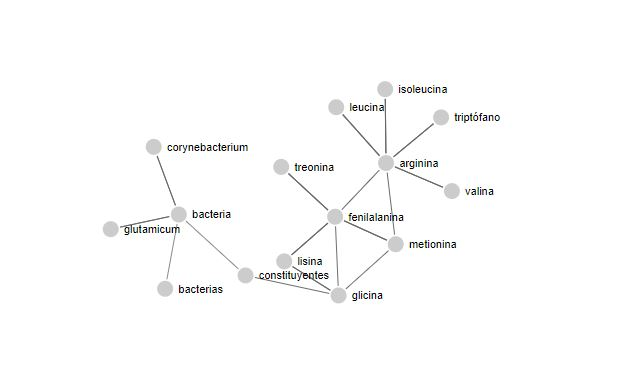
\includegraphics[width=0.8\textwidth]{grupo25}
%\caption{Grafo  relaciones temáticas grupo 17}
%\label{fig:grupo25}
%\end{figure}
%
%En el grupo 18 se encuentran trabajos relacionados con temáticas temáticas afines a administración, economía y finanza empresarial.
%
%En el grupo 19 se encuentran trabajos relacionados a temáticas sociales, desarrollo humano sostenible, desarrollo económico social, derecho internacional humanitario y políticas comunitarias.
%
%En el grupo 20 se encuentran trabajos de grado de la facultad de artes, referentes a temáticas culturales, artesanías e  historia del arte.
%
%En el grupo 21 se encuentran trabajos relacionados a la facultad de ciencias económicas y administrativas los cuales involucran temáticas de comercio exterior, aduanas, exportaciones, impuestos, empresas, fiscalización y estudios de mercados.
%
%
%En el grupo 22 se encuentran trabajos de grado relacionados con planes de ordenamiento  territorial   y ecoturismo tal como se observa en la figura \ref{fig:ordenaminetoimg}.
%
%
%\begin{figure}[H]\centering
%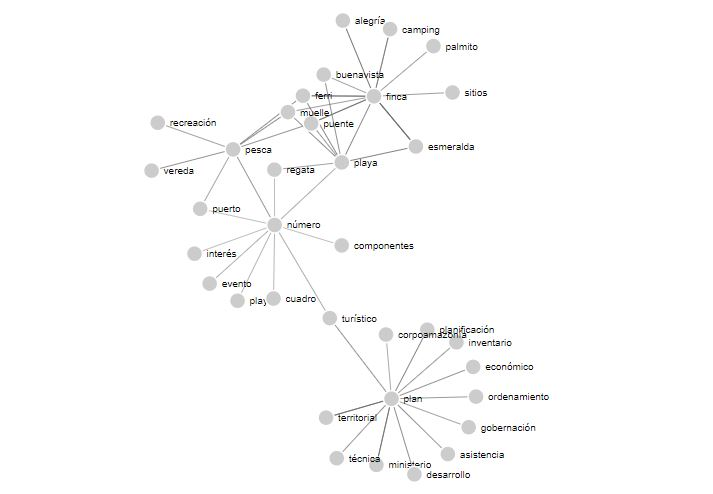
\includegraphics[width=1\textwidth]{ordenaminetoimg}
%\caption{Grafo relaciones temáticas grupo 22 }
%\label{fig:ordenaminetoimg}
%\end{figure}
%
%En el grupo 23 se encuentran trabajos de grado de la facultad de ciencias agrícolas, específicamente del programa de ingeniería agronómica, relacionando temáticas referentes a estudios de variedades de especies de granos, tubérculos, plantas y técnicas de comparación de diferentes tratamientos agronómicos mediante pruebas de Tukey y validaciones estadísticas
%como se representa en la figura \ref{fig:grupo25}.
%\begin{figure}[H]\centering
%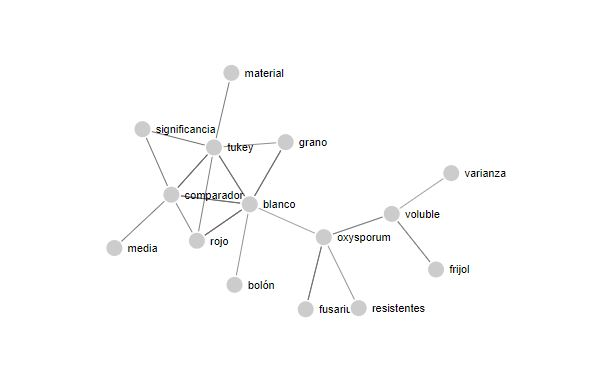
\includegraphics[width=0.8\textwidth]{grupo28}
%\caption{Grafo  relaciones temáticas grupo 23}
%\label{fig:grupo25}
%\end{figure}
%
%
%En el grupo 24 se encuentran trabajos relacionados con medicina veterinaria, en la figura \ref{fig:grupo7} se aprecia relaciones entre enfermedades causadas por las bacterias babesia y  anaplasma en equinos.
%
%\begin{figure}[H]\centering
%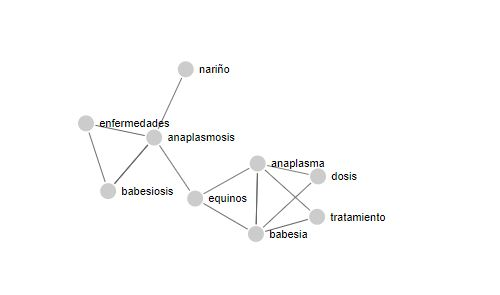
\includegraphics[width=0.8\textwidth]{grupo7}
%\caption{Grafo  relaciones temáticas grupo 24 }
%\label{fig:grupo7}
%\end{figure}
%
%En el grupo 25 se encuentran trabajos de grado relacionados con proyectos de priorización de áreas ambientales, caracterización de sistemas agroforestales, investigación de especies y reservas naturales.  %%
%
%En el grupo 26 se encuentran trabajos de grado relacionados con música.
%
%En el grupo 27 se encuentran trabajos relacionados con temáticas pedagógicas para la educación. 
%\begin{figure}[H]\centering
%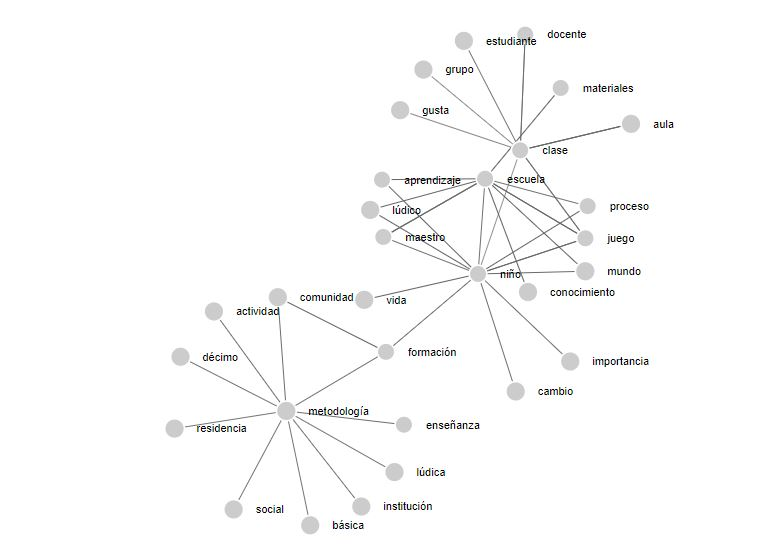
\includegraphics[width=0.8\textwidth]{grupo8}
%\caption{Grafo  relaciones temáticas grupo 27 }
%\label{fig:grupo8}
%\end{figure}
%
%En la figura \ref{fig:grupo8} podemos observar relaciones contextuales complementarias del grupo 27 tales como: escuela, maestros , aulas de clase, estrategias y metodologías didácticas de aprendizaje basadas en lúdicas y juegos para niños estudiantes de básica  primaria.
%
%En el grupo 28 se encuentran trabajos de grado relacionados al programa de administración empresas, referentes a estudios del clima organizacional, talento humano, selección de personal, control interno y procesos de gestión y calidad en las empresas.
%
%En el grupo 29 se encuentran trabajos de grado del programa de Psicología, relacionados con factores de riesgo en adolencetes causantes de suicidio, identificación de ideas suicidas como se describe en la figura \ref{fig:grupo14}.
%\begin{figure}[H]\centering
%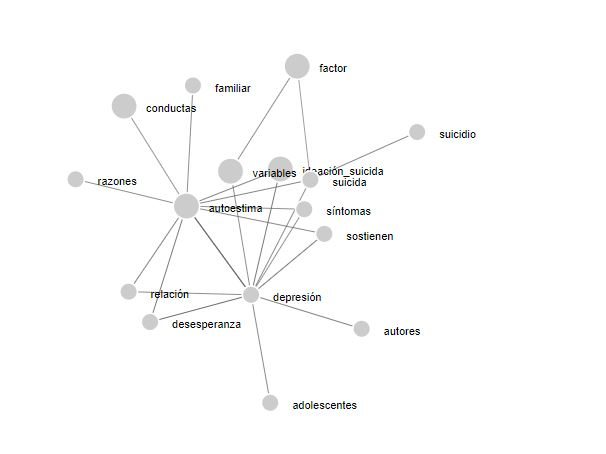
\includegraphics[width=0.8\textwidth]{grupo19}
%\caption{Grafo  relaciones temáticas grupo 29 }
%\label{fig:grupo19}
%\end{figure}
%
%En el grupo 30 se encuentran trabajos relacionados al programa de ingeniería de sistemas, particularmente al área de descubrimiento de conocimiento en base de datos, desarrollo de herramientas bajo el gestor Postgresql, algoritmos de minería de datos, clasificación, agrupación, reglas de asociación y temáticas de software y manejo de información.
%
%\begin{figure}[H]\centering
%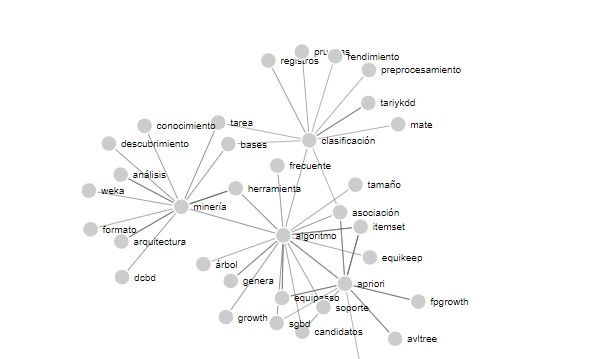
\includegraphics[width=0.8\textwidth]{grafotarykdd}
%\caption{Grafo  relaciones temáticas grupo 30 }
%\label{fig:tarygradfo}
%\end{figure}
%
%En las figuras \ref{fig:tarygradfo}  se muestra el grafo conceptual generado por el modelo Word2vec de los trabajos de grado respectivos al  grupo 30. Donde se pueden establecer vínculos entre conceptos dentro de minería de datos, descubrimiento de conocimiento, algoritmos de clasificación y asociación tales como equipasso, fpgrowth, entrenamiento de  árboles  de decisión, a priori e itemsets frecuentes.
%
%En el grupo 31 se encuentran trabajos de grado relacionados con las ciencias pecuarias, producción acuícola y comparación de dietas en cultivos de peces.


\section{Comparación  de los dominios de conocimiento entrenados.}

Para saber que modelo distingue mejor las áreas de conocimiento de los documentos  estructurados por el método  Doc2vec, se evalúa y compara cada clasificador entrenado.
  Se utilizaron las métricas de accuracy (exactitud) y f1 para los conjuntos de entrenamiento (70\%),   testing (30\%) y el método de validación cruzada (k fold=5). La accuracy expresa la cantidad de casos correctamente clasificados sobre el total, y F1 (F-Score o medida-F) la medida de precisión que tiene un test, ponderando la precisión y la exhaustividad, la medida f1 se calculó con la fórmula Macro-averaged F-Measure explicada  en  \cite{ozgur2005text}.

\begin{figure}[H]
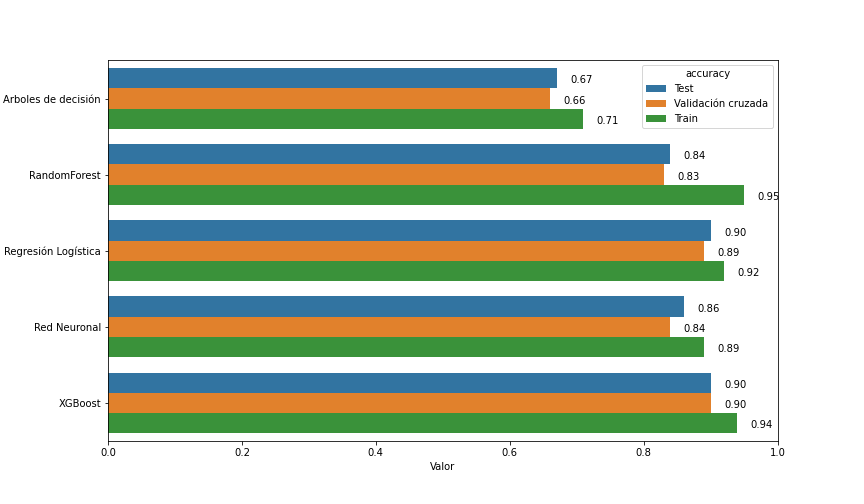
\includegraphics[width=0.5\textwidth ,height=350]{clasificadoresA}
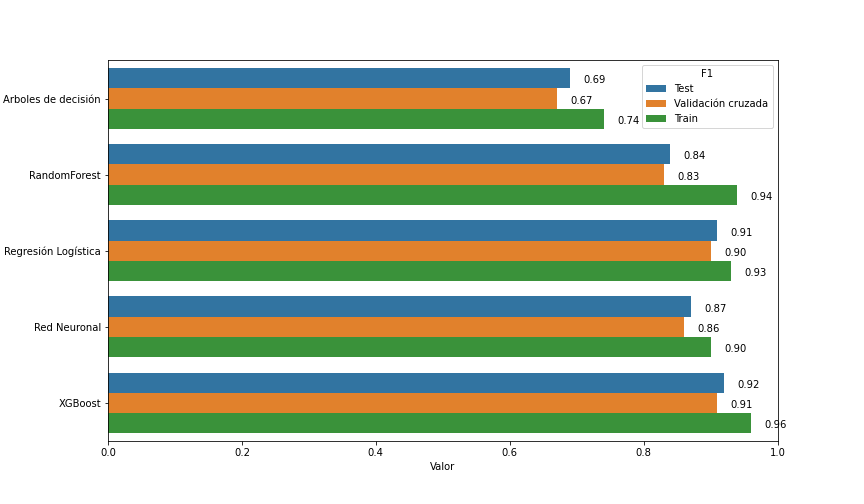
\includegraphics[width=0.5\textwidth ,height=350]{clasificadoresF1}
\caption{Comparativa de los clasificadores entrenados }
\label{fig:clasificadoresA}
\end{figure}

En la figura \ref{fig:clasificadoresA} se aprecia que los modelos sufren un ligero sobreajuste en el conjunto de entrenamiento, el modelo RandomForestes el más sobre ajustado, ya que baja notoriamente su performance en el conjunto de testing y el método de validación cruzada.
El único clasificador que obtiene resultados notablemente más bajos es el árbol de decisión , mientras que los otros obtienen puntajes por encima del 80\%.
Los mejores modelos en términos de Accuracy y F1 en los conjuntos de validación son Xgboost y Regresión logística; a pesar de que el modelo Xgboost está un poco más sobre ajustado al conjunto de entrenamiento, es el que obtuvo mejores resultados en test, por tanto es el modelo utilizado  en el algoritmo \ref{alg:maskanita1} y para la clasificación  de los nuevos documentos que ingresen al repositorio. En \cite{seyfiouglu2017hierarchical} se obtiene una precisión general del 92,5\% utilizando el modelo XGBOOST bajo un corpus estructurado con Doc2vec para una clasificación binaria, para la clasificación de 12 categorías obtuvieron una precisión general del 71,16\%, la diferencia con respecto a la precisión obtenida en esta investigación puede darse por los dominios de conocimiento entre repositorios y también los métodos de obtención de las categorías a entrenar; ya que en este  método propuesto se obtuvo la clase a partir del agrupamiento validado con el coeficiente de silhouette, por tanto la adopción de técnicas complejas no siempre garantizan el logro de obtener mejores resultados y  pueden variar de acuerdo a los repositorios textuales que se pretendan investigar.

\begin{figure}[H]\centering
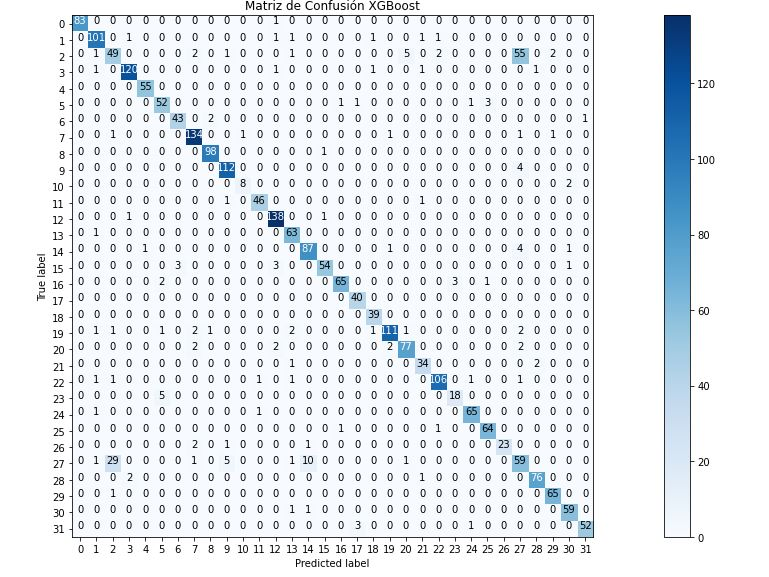
\includegraphics[width=0.8\textwidth]{matrixbost}
\caption{Matriz de confusión modelo Xgboost para el conjunto de testing}
\label{fig:mconf}
\end{figure}

En la figura \ref{fig:mconf} se muestra la matriz de confusión en testing para el mejor modelo de Xgboost. El porcentaje de casos correctamente clasificados es de 90\%; los casos mal clasificados con un desvío de clase entre los grupos 2 y 27 se debe a que existe correlación entre los dominios de conocimiento, el algoritmo  \ref{alg:maskanita1}  toma las probabilidades asignadas por el modelo Xgboost y busca documentos similares entre los grupos con más alta probabilidad.

Se reproduce un caso a modo de ejemplo del algoritmo \ref{alg:maskanita1}. Se trata de un nuevo trabajo que contenga ''perceptrones multicapa backpropagation''. El algoritmo predice que este tema se relaciona con el grupo 11 con una probabilidad de 99\% y los documentos más similares dentro del grupo son: 
''Detección automática de registros sísmicos asociados al comportamiento del volcán galeras haciendo uso de redes neuronales artificiales'' con una similitud de 0.84 y ''Diseño e implementación de un sistema clasificador prototipo de granos de café por tamaño y color'' con una similitud de 0.82.





